% method
\def\A{\ensuremath{A}}
\def\E{\ensuremath{E}}
\def\C{\ensuremath{C}}

\def\AW{\ensuremath{A_W}}
\def\EW{\ensuremath{E_W}}
\def\AZ{\ensuremath{A_Z}}
\def\EZ{\ensuremath{E_Z}}

\def\Wall{\ensuremath{\Wminus+\Wplus}}

The objective of this analysis is to measure the cross-section of \Wboson\ bosons decaying into a muon and a neutrino (in other words, the total production cross-section of the \Wboson, times its \Wmn\ branching ratio). The overall plan of attack can be summarized as follows:
\begin{itemize}
\item Starting with raw data events from the LHC, various cuts are applied to remove events that are inconsistent with the \Wmn\ process.
\item The surviving events are still contaminated with backgrounds that may mimic the experimental footprint of real \Wboson events. These backgrounds are estimated (from Monte-Carlo simulation or through data-driven methods) and subtracted from the pool of candidates.
\item Using \Wmn\ Monte-Carlo, the background-subtracted signal counts are adjusted for detector efficiency and resolution effects, and optionally extrapolated to a more inclusive phase space (for instance, to cover regions not directly instrumented by the detector). This procedure is called ``unfolding'' and produces a detector-independent measurement that can be directly compared against theoretical predictions.
\item The above steps are repeated several dozen times - once for each systematic variation - to assess the impact of these variations on the final measurement.
\end{itemize}

\section{The ATLAS Coordinate System}
The proton-proton interaction point serves as the pivot for the common coordinate system used at ATLAS. The z-axis runs along the beam line and the $x-y$ plane, which is perpendicular to the beam, defines the transverse plane. Transverse momentum $p_T$ is the projection of the particle momentum on the transverse plane, as illustrated in Fig.~\ref{fig:defetapt}(a). $\phi$ is the azimuthal angle in the transverse plane, while $\theta$ is the polar angle with respect to the beam axis. Transverse energy $E_T$ of a particle is defined as $E \cdot \sin \theta$. Missing transverse energy $\met$ quantifies the imbalance in the vectorial sum of transverse energies of all objects measured by the detector, which serves as a proxy for the $p_T$ of the particles that escape detection. Pseudorapidity $\eta$ is a monotonic transformation of the polar angle defined by the following formula:
$$\eta = -\log\biggl(\tan\frac{\theta}{2}\biggr)$$
The value of $\eta$ for different values of $\theta$ is illustrated in Fig.~\ref{fig:defetapt}(b).

\begin{figure}[phtb]
  \begin{center}
        \subfigure[Transverse momentum $p_T$]{%
          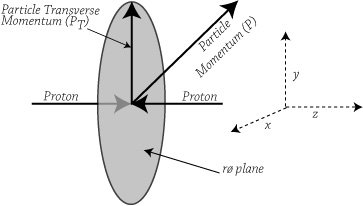
\includegraphics[width=0.44\textwidth]{method/fig/PT}
        }
        \subfigure[Pseudorapidity $\eta$]{%
          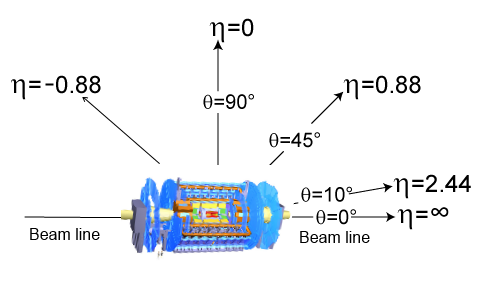
\includegraphics[width=0.44\textwidth]{method/fig/pseudorapidity}
        } 
 \caption{ Geometric illustration of the transverse momentum (left), polar angle and pseudorapidity (right). }
 \label{fig:defetapt}
 \end{center}
\end{figure}

\section{Integrated, Single and Double-Differential Measurements}
The \Wmn\ cross-sections are reported in three different binnings: integrated, single- and double-differential. All cross-sections are measured separately for \Wplus\ and \Wminus.

The integrated cross-section is unbinned and provides the production rate in the phase space covered by the detector, as well as in the full phase space. The single-differential cross-section is provided in bins of the absolute value of the muon pseudorapidity. The $|\eta|$ dependence of the cross-section provides valuable information about the proton structure, as elaborated in Sec.~\ref{chap:pdf_theory}. The double-differential cross-section further splits the measurement into bins of the transverse momentum of the muon in order to test whether the $p_T$ dependence of the cross-section is modeled properly by fixed-order theory calculations.

\section{Cross-Section Formula}
\label{sec:xsec_formula}
Mathematically, the cross-section can be derived from the following formula:
\begin{equation}
 \sigma \times BR =
 \frac{N - B}{\C \cdot \E \cdot \A \cdot L_{int}  \cdot \Gamma} \,,
\label{eq:WZxsec}
\end{equation}
where
\begin{itemize}
\item $N$ is the number of \Wboson\ candidate events in data,
\item $B$ is the number of background events,
\item $L_{int}$ is the integrated luminosity (total amount of collected data)
\item $\Gamma$ is the bin width. For differential measurements (but not integrated), the cross-sections are traditionally quoted per-unit of pseudorapidity or momentum, which allows for easier comparison of the values in variable-width bins.
\item \C\ is the factor used to correct for detector efficiency and resolution effects. It is derived from Monte-Carlo (MC below) and translates the cross-sections from ``reconstruction level'' to ``generator level'', which is independent of the specific features of the detector and can be defined in purely theoretical terms for a given fiducial phase space. 
    \begin{equation}
      \C = \frac{N_\mathrm{MC, rec, fiducial}}{N_\mathrm{MC, gen, fiducial}}\,. \label{eq:c}
    \end{equation}
 The \C\ factor does not perform any fiducial extrapolation: the same fiducial cuts ($p_T$, $\eta$, etc) are applied at the generator level as at the reconstruction level. However, it includes the effects of QED final state radiation, or FSR (radiation of additional photons off the muon) by correcting all muons down to a pre-FSR ``Born'' level.
\item \E\ is the factor used to perform a small theoretical extrapolation from $|\eta|<2.4$ to $|\eta|<2.5$. This is done for two reasons: to align \Wmn\ cross-sections to a common fiducial volume used in the combination with the \Wen\ channel, and to facilitate comparison with theoretical predictions, which were produced with $|\eta|<2.5$.
    \begin{equation}
      \E = \frac{N_\mathrm{MC, gen, fiducial}}{N_\mathrm{MC, gen, fiducial\_extrap}}\,.
    \end{equation}
\item \A\ is a theoretical acceptance factor used to extrapolate cross-sections to the full phase space volume before any cuts. It is only applied to the integrated cross-section.
    \begin{equation}
      \A = \frac{N_\mathrm{MC, gen, fiducial\_extrap}}{N_\mathrm{MC, gen, all}}\,.
    \end{equation}
\end{itemize}

\section{Phase Space and Binning}
\label{method:fid:space}
Integrated, single- and double-differential cross-sections are measured in the phase space instrumented by the ATLAS detector. In other words, the cuts applied at the generator level mimic the \Wmn\ selection criteria used at the reconstruction level. These cuts, along with the differential bin boundaries, are summarized in Tab.~\ref{tab:ExpFidW}. The $|\eta|$ bins have variable widths and are chosen to follow the geometrical features of the detector. Definitions of $\eta$ and $p_{T}$ were given above; \mt\ is the transverse mass of the \Wboson\ candidate, which is defined as:
$$m_{T}^2 = 2 \cdot p_{T, \mu} \cdot p_{T, \nu} \cdot (1 - \cos\phi_{\mu, \nu})$$
, where $\phi_{\mu, \nu}$ is the azimuthal angle between the muon and the neutrino.
The fiducial phase space is subsequently expanded from $|\eta|<2.4$ to $|\eta|<2.5$ to facilitate combination with the \Wen\ channel and with theoretical predictions. This is accomplished with the \E\ extrapolation factors, as described in Sec.~\ref{sec:xsec_formula}.

The integrated measurement is additionally extrapolated to the full phase space using the acceptance factors (\A).

\begin{table}
  \begin{tabular}{|l|l|}
    \hline\hline
   \multicolumn{2}{|c|}{\Wmn\ Experimental Phase Space} \\\hline
   Integrated &
   \parbox{0.87\textwidth}{
     \begin{itemize}[noitemsep,topsep=5pt,parsep=0pt,partopsep=0pt]
     \item Separately $W^+$ and $W^-$
     \item $|\eta|<2.4$
     \item $p_{T, \nu} >25\gev$
     \item $\mt>40\gev$
     \item $p_{T_\mu} > 25\gev$
     \end{itemize}
   }\\\hline
   Differential & 
   \parbox{0.87\textwidth}{
     \begin{itemize}[noitemsep,topsep=5pt,parsep=0pt,partopsep=0pt]
     \item Separately $W^+$ and $W^-$
     \item $p_{T, \nu} >25\gev$
     \item $\mt>40\gev$
     \item $d\sigma/d|\eta_\mu|$ in 11 $|\eta_\mu|$ bins for $p_{T_\mu} > 25\gev$ with bin boundaries at:\\
       $|\eta_\mu|$ : 0.0, 0.21, 0.42, 0.63, 0.84, 1.05, 1.37, 1.52, 1.74, 1.95, 2.18, 2.4
     \item $d\sigma/d|\eta_l|\,dp_{T,\mu}$ in $11 \times 7$
       $|\eta_\mu| \times p_{T, \mu}$ bins with bin boundaries at:\\
       $|\eta_\mu|$ :
       0.0, 0.21, 0.42, 0.63, 0.84, 1.05, 1.37, 1.52, 1.74, 1.95, 2.18, 2.4\\
       $p_{T,\mu}$ : 20, 25, 30, 35, 40, 45, 50, $\infty$ $[\gev\,]$\\
     \end{itemize}
   }\\\hline
 \end{tabular}
 \caption{ Definition of fiducial phase space for \Wmn, mimicking the experimental cuts applied at the reconstruction level.}
 \label{tab:ExpFidW}
\end{table}

\section{Bin Migrations}
\label{sec:puritystability}
It is possible that an event generated in a particular bin ends up reconstructed in another bin. For example, due to imperfect detector resolution, the transverse momentum of a muon may be reconstructed with a slightly higher value, putting the event into a subsequent $p_T$ bin. The magnitude of bin migrations can be understood in terms of the purity $P^{i}$ and stability $S^{i}$ in each bin $i$:

\begin{equation}
P^{i} = \frac{N^{i}_{\text{rec\&gen, all fiducial cuts}} }{ N^{i}_{\text{rec, all fiducial cuts}} }, \; \;
S^{i} = \frac{N^{i}_{\text{rec\&gen, all fiducial cuts}} }{ N^{i}_{\text{gen, all fiducial cuts}} },
\label{Eq:PurityStability}
\end{equation}
where
\begin{itemize}
\item $N^i_{\text{rec, all fiducial cuts}}$~--- the sum of events reconstructed in bin $i$,
\item $N^i_{\text{gen, all fiducial cuts}}$~--- the sum of events generated in bin $i$,
\item $N^i_{\text{rec\&gen, all fiducial cuts}}$~--- the sum of events which were both generated and reconstructed in bin $i$.
\end{itemize}

The effect of bin migrations on the \C\ factor can be taken into account through an iterative Bayesian unfolding procedure~\cite{Adye:arXiv1105.1160}. This is further described in Sec.~\ref{sec:appmigrations}.
